\section{Results}

\sepfootnotecontent{sf:supExecQueryShapeContainment}{
    The execution times with the other shapes are lower and also negligible. 
    Tables of results are available online with the supplementary materials.
}

\begin{figure}[h]
    \centering
    \includegraphics[width=0.45\linewidth]{analysis/artefact/variation_approach/reduction_query_execution_time}
    \caption{
        This figure compares the type index with the LDP approach against other approaches.
        The shape index approach performs better than the other approaches except with S4.
        The shape index can also answer queries from the S7V3, which the plot cannot capture.
    }
    \label{fig:compApproach}
\end{figure}

\begin{figure}[htbp]
    \centering
    % First figure
    \begin{minipage}{0.32\textwidth}
        \centering
        \includegraphics[width=\linewidth]{analysis/artefact/variation_percentage_shape_index/reduction_query_execution_time}
        \caption*{a) Percentage of shape index in the network}
        \label{fig:varPercentShapeIndex}
    \end{minipage}
    \hfill
    % Second figure
    \begin{minipage}{0.32\textwidth}
        \centering
        \includegraphics[width=\linewidth]{analysis/artefact/variation_percentage_entry_shape_index/reduction_query_execution_time}
        \caption*{b) Percentage of entries having open shapes}
        \label{fig:varPercentEntries}
    \end{minipage}
    \hfill
    % Third figure
    \begin{minipage}{0.32\textwidth}
        \centering
        \includegraphics[width=\linewidth]{analysis/artefact/variation_detail_shape/reduction_query_execution_time}
        \caption*{c) Level of detail of the shapes}
        \label{fig:varShapeDetail}
    \end{minipage}

    % General caption
    \caption{Setups with less shape index information tend to perform worse where the shape index perform
    better against the other approaches in similar relative proportions.
    %We also observe that having a higher percentage of open shapes have generally a less negative impact than 
    %on performance compared to having a lower percentage of datasets without shape indexes.
    }
    \label{fig:three_figures}
\end{figure}

\begin{figure}[htbp]
    \centering
    % First figure
    \begin{minipage}[t]{0.45\textwidth}
        \centering
        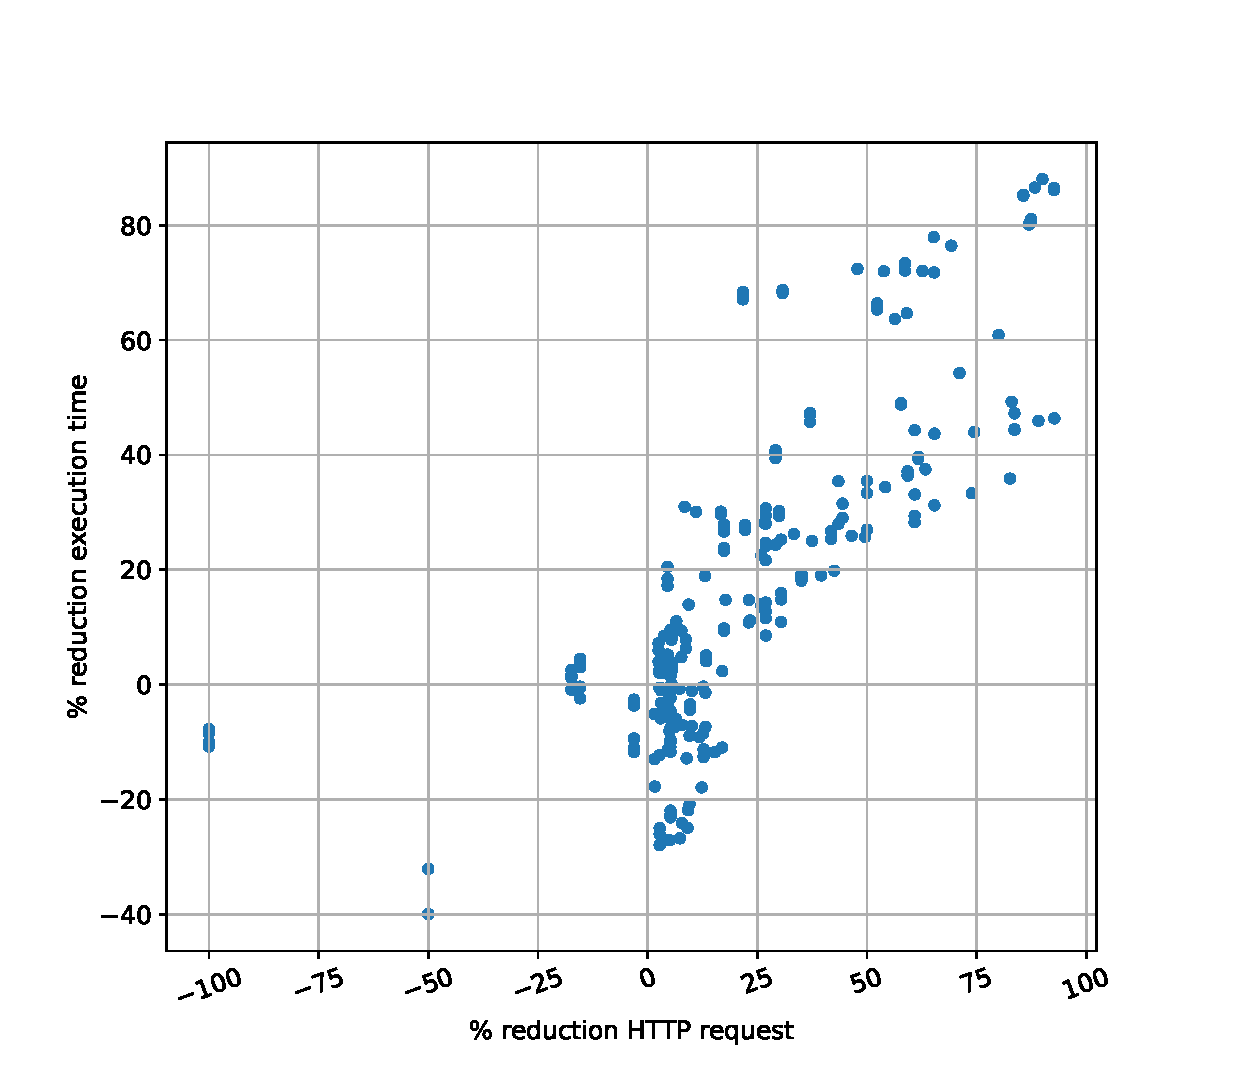
\includegraphics[width=\linewidth]{analysis/artefact/http_req_exec_time_relation/http_req_exec_time_cor_better}
        \label{fig:http_req_exec_time_cor_better}
    \end{minipage}
    \hspace{0.05\textwidth}
    % Second figure
    \begin{minipage}[t]{0.45\textwidth}
        \centering
        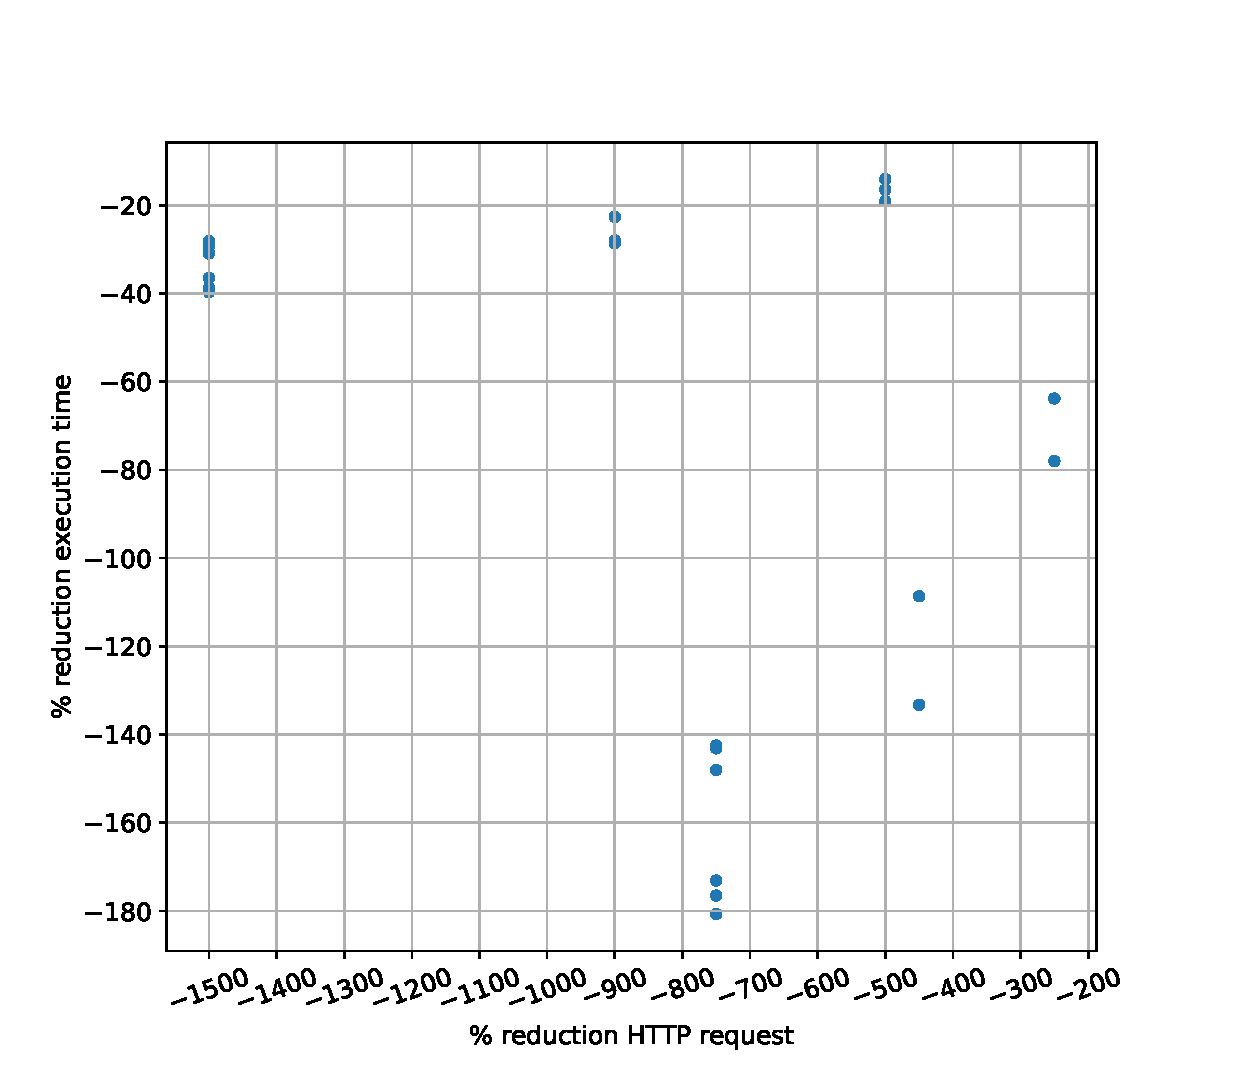
\includegraphics[width=\linewidth]{analysis/artefact/http_req_exec_time_relation/http_req_exec_time_cor_worse}
        \label{fig:http_req_exec_time_cor_worse}
    \end{minipage}

    % General caption
    \caption{On the left is the distribution of reduction of HTTP requests by reduction of execution time.
    The data show two regimes, one where there is a reduction or a slight increase of HTTP requests on the right figure and one where there is a large increase of HTTP requests on the left.
    The overall distribution is linear with a PCC of 0.55 and a p-value of 6.18E-35.}
    \label{fig:http_req_exec_time_cor}
\end{figure}

Figure~\ref{fig:compApproach} shows that the shape index is able, with multiple queries, to perform better than the state-of-the-art.
The queries that performed best were those where the number of HTTP requests decreased the most.
In the annex, plots of the number of HTTP requests by query template are displayed, and the statistical significance for each query instance is evaluated.
Queries templates such as D6 and D7 show no reduction because those queries request every document following the shape containing interesting information of the datasets of the network, thus
our approach is unproductive and can even cause overhead in the calculation.
We notice that query template S4 with the shape index performed worse, with an increase in query execution time of up to 2.80 times.
The reason is that with the other approaches, only the reachability \texttt{Cmatch} was used to obtain completeness, so the structural properties of the dataset were not used; with the shape index, we always force the usage of this property of the datasets leading to extra HTTP requests and more processing.
However, this query was already fast, with the state-of-the-art approach being executed in approximately 0.30\% of the timeout.
However, these results still show a category of network and queries for which our approach is not suited.

The empirical evaluation of the query-containment algorithm shows that its execution with the more detailed shapes of our experiment is negligible, with a maximum execution of 4.655 ms (0.0039\% of the timeout), as presented in table~\ref{tab:queryShapeContainmentEval}.~\sepfootnote{sf:supExecQueryShapeContainment}
This result is expected because the algorithm's time complexity is ("TO INSERT"), and the experiments' shapes and queries are small, not deeply nested instances.
This shows that most of the overhead is not this algorithm but is probably the state retention for the pruning reachability criteria and the parsing of the index into an internal object.
Figure~\ref{fig:http_req_exec_time_cor} shows that without an increase in the number of HTTP requests, the performance can increase up to 10\%.


To determine the relationship between the reduction of HTTP requests and the reduction of query execution time as compared to the reachability using the type index and the LDP specification (the state-of-the-art),
we aggregated those data from each experiment and plotted the results, which can be seen in Figure~\ref{fig:http_req_exec_time_cor}.
The relationship between HTTP request and query execution time can be divided into two regimes.
In the first regime (left figure), where the shape index approach reduces the number of HTTP requests, we notice a positive linear correlation with a
Pearson correlation coefficient (PCC) of 0.83 with a high statistical significance (p-value 2.94E-93).
We can also notice that below a ratio of approximately 0.83, the shape index approach did not guarantee a reduction in query execution time.
In the second regime (right figure), the shape index increases the number of HTTP requests.
We notice a weaker positive linear correlation with a PCC of 0.43, with a high but far lower statistical significance (p-value 1.16E-04) and fewer samples.
The overall correlation between reducing HTTP requests and query execution time is positively linear, with a PCC of 0.55 and a high statistical significance (p-value 6.18E-35).
It is difficult to explain why the data operate in two regimes. 
A possible explanation can simply be the lack of samples when the shape index approach performs poorly.
However, we can also notice that the relationship between the two variables in the first regime is close to one-on-one, whereas, in the second regime, the number of HTTP requests has less of an impact.
This observation can lead us to question how complex the queries are in that regime; we can notice that the queries where the shape index increases vastly in the number 
of HTTP requests are the queries from the S4 template. 
However, this query was already answered quickly and consisted of only four triple patterns and a union statement (with the alternative property), so the query is simple. 
Thus, it is possible that the number of HTTP requests has less of an impact because it is easier for the engine to perform the join operation upon reception of the data as opposed to more complex queries.
With this current experiment, it is not possible to answer this question.
